\documentclass[../thesis.tex]{subfiles}
% !TeX spellcheck = fr_FR

\begin{document}
    \chapter{Matériel et données}
    \label{chap:mat-and-data}
    
    \section{Les sites expérimentaux}
    
    \subsubsection{Expérimentations en micro-parcelles}
    \label{sec:premiere-xp}
    
    Une parcelle expérimentale a été mise en place à AgroSup Dijon (semée le 01/06/2019), afin de réaliser des acquisitions à différents stades de développement des cultures et des adventices (figure \ref{fig:04-parcelle-inra} gauche) et de préparer le challenge. Cette parcelle expérimentale a été découpée en 4 micro-parcelles de \SI{9}{m} par \SI{60}{cm} pour 4 cultures (de bas en haut : maïs, orge, féverole, trèfle) et trois rangs de cultures ont été semés pour chaque bande. Les adventices ont poussé naturellement et chaque bande a également été divisée en 3 modalités de désherbage de \SI{3}{m} (faible $<\SI{20}{\percent}$, partiel $40-\SI{60}{\percent}$ et aucun), dans le but de montrer l'impact de la segmentation sur le potentiel de discrimination. La parcelle a été préparée et semée manuellement.
    
    %\newpage
    \subsubsection{Expérimentations en parcelles agricoles}
    \label{sec:grande-xp}
    
    Des acquisitions en parcelles agricoles ont été réalisées dans le cadre du challenge RoSE, avec le consortium ROSEAU. La parcelle expérimentale est gérée par OPEROSE \cite{ChallengeRoSE}, équipe s'occupant des aspects opérationnels (entretiens, itinéraires techniques, \dots) de l'ANR Challenge RoSE, localisée sur le site INRAE, Domaine des Palaquins, Montoldre dans l'Allier (figure \ref{fig:04-parcelle-inra} droite). Cette équipe organise les campagnes d'évaluations, permettant de mesurer la progression des performances et la maturité technologique des équipes au sein de l'ANR RoSE. 
    
    La parcelle expérimentale est divisée en plusieurs rangs de tests, dont un rang de maïs (inter-rang $\SI{75}{cm} - \SI{80}{cm}$) et un rang de haricot (inter-rang $\SI{15}{cm} - \SI{37}{cm}$) dédiés à la tâche de détection. Des adventices naturelles sont présentes, comme la matricaire, la renouée des oiseaux, le chénopode, la sétaire, la morelle, ou la digitaire. Des adventices ``modèles'' ont été semées dans l'intra-rang, qui comporte de la moutarde, de la vesce, du trèfle, des lentilles, du ray-grass, de l'avoine, de la fétuque, et des dactyles.
    
    \vfill
    \begin{figure}[H]
        \centering
        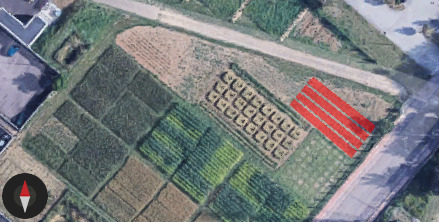
\includegraphics[height=4cm]{img/material/parcelle-inra}
        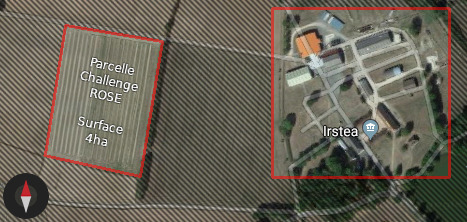
\includegraphics[height=4cm]{img/material/parcelle-xp}
        \caption{Parcelle pour les premières expérimentations (rouge) à gauche et parcelles utilisées par le consortium ROSEAU (droite)}
        \label{fig:04-parcelle-inra}
    \end{figure}
    \vfill
    \null
    
    %\begin{figure}[H]
    %    \centering
    %    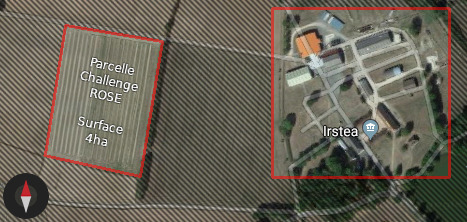
\includegraphics[width=0.6\linewidth]{img/material/parcelle-xp}
    %    \caption{Parcelles utilisées par le consortium ROSEAU}
    %    \label{fig:04-parcelle-xp}
    %\end{figure}
    
    \newpage
    \section{Capteur optique}
    
    \par Toutes les données ont été acquises avec la caméra multispectrale  Airphen de la société Hiphen (Avignon, France). Ceci permettra de comparer plus facilement le niveau de discrimination de nos critères, en fonction des situations. Le système optique dispose de 6 capteurs optiques disposés en damier (figure \ref{fig:04-airphen-detail4}). Chacun capteur se compose d'un CCD $4/3''$ (Taille : $\SI{4.8}{mm} \times \SI{3.6}{mm}$) et d'une focale de \SI{8}{mm} et est équipé d'un filtre interférentiel de \SI{10}{mm}. Les 6 images acquises ont une taille de $1280\times\SI{960}{px}$ et sont enregistrées au format TIFF avec un codage entier sur \SI{12}{bits}.
    
    \begin{figure}[H]
        \centering
        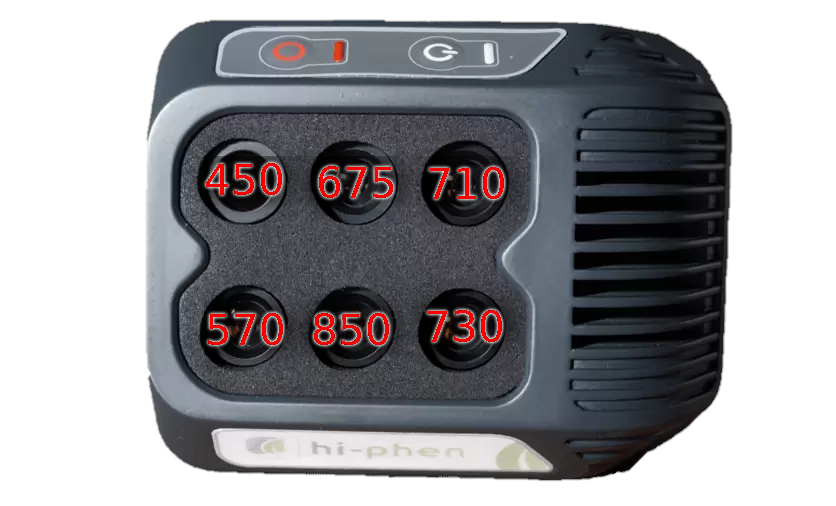
\includegraphics[width=0.45\linewidth]{img/preprocessing/airphen-detail4}
        \caption{Système optique de la caméra Airphen (Société Hiphen, France)}
        \label{fig:04-airphen-detail4}
    \end{figure}
    
    Pour caractériser la végétation, le choix des bandes spectrales retenues pour les filtres interférentiels a été défini lors d'une étude précédente, conduite durant la thèse de \cite{MRNL2016}. Le travail effectué consistait à chercher les longueurs d'onde optimales pour la discrimination culture/adventices. Plusieurs méthodes ont été utilisées et une synthèse a permis de sélectionner les filtres les plus discriminants. Ils sont respectivement centrés sur 450, 570, 675, 710, 730 et \SI{850}{nm} (figure \ref{fig:04-sepctral-response}). Ces longueurs d'onde seront utiles pour le calcul des indices de végétation, la segmentation et l'extraction des informations pour la discrimination culture/adventices.
    
    \begin{figure}[H]
        \centering
        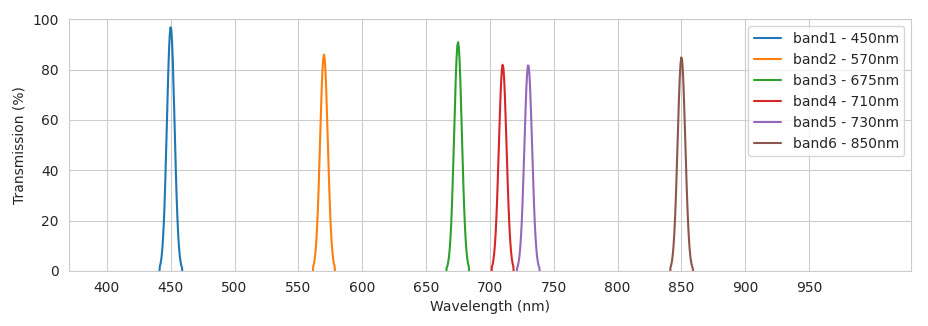
\includegraphics[width=\linewidth]{img/material/spectral-response-plt}
        \caption{Réponse spectrale des 6 filtres interférentiels placés devant les capteurs de la caméra multispectrale}
        \label{fig:04-sepctral-response}
    \end{figure}
    
    %\newpage
    \section{Jeux de données}
    \subsection{Campagnes d'acquisition}
    
    \paragraph{Micro-parcelles}
    
    Un premier jeu de données a été acquis afin de tester et d'élaborer les différentes étapes de la chaîne fonctionnelle. La caméra multispectrale est embarquée sur une brouette thermique modifiée afin d'être dans les mêmes conditions expérimentales que le challenge ROSE. Les acquisitions ont été réalisées au mois de Juillet à quatre dates espacées d'une semaine. Le tableau \ref{tab:04-acquisition-source} synthétise ces acquisitions. Cependant, durant cette période, la sécheresse a beaucoup impacté les cultures et les adventices ne permettant pas d'utiliser ces données pour montrer l'impact de la segmentation sur le potentiel de discrimination. Certaines de ces données ont néanmoins été utilisées pour calibrer la caméra et établir des indices de végétation optimaux. Notons que le maïs, qui est absent du tableau \ref{tab:04-acquisition-source}, n'a simplement pas levé. Finalement, les féveroles à la quatrième acquisition étaient en sénescence.
    
    \begin{table}[H]
        \centering
        \begin{tabular}{l c c c c}
            \hline \textbf{Culture} & \textbf{10/07/2019} & \textbf{17/07/2019} & \textbf{24/07/2019} & \textbf{31/07/2019} \\ \hline
            Orge 1 		& 61 & 65 & 53 & 40 \\
            Orge 2 		& 74 & 58 & 70 & 64 \\ \hline
            Féverole 1  & 51 & 66 & 51 & -- \\
            Féverole 2  & 90 & 68 & 70 & -- \\ \hline
            Trèfle 1    & 68 & 78 & 48 & 48 \\ 
            Trèfle 2    & 62 & 73 & 81 & 69 \\ \hline
        \end{tabular}
        \caption{Dates d'acquisition, cultures et nombre d'images acquises}
        \label{tab:04-acquisition-source}
    \end{table}
    
    \paragraph{Challenge RoSE}
    
    Pour les acquisitions réalisées avec le consortium ROSEAU, la caméra multispectrale Airphen a été embarquée sur le robot PUMAGRI (Figure \ref{fig:04-robot-xp}) de la société SITIA. C'est un robot autonome destiné à la gestion localisée des adventices disposant de différents outils pour le désherbage (mécanique ou chimique). Dans le cadre de cette thèse, seule la partie détection des adventices est évaluée. Le challenge s'est déroulé sur trois ans entre 2018 et 2021, avec une campagne d'acquisition la première année, et deux les suivantes. Le nombre d'acquisitions par culture est synthétisé sur le tableau \ref{tab:04-acquisition-challenge}. Cette thèse ayant commencé en Décembre 2018, nous n'avons pas participé au premier challenge. De plus, le challenge 5 devant se dérouler en juin a finalement du être repoussé à cause des conditions météorologiques.
    
    \begin{table}[H]
        \centering
        \begin{tabular}{l c c c c}
            %\hline \textbf{Culture} & \textbf{Challenge 3} & \textbf{Challenge 4} & \textbf{Challenge 5} & \textbf{Challenge 6} \\
            \hline \textbf{Culture} & \textbf{25/09/2019} & \textbf{10/06/2020} & \textbf{23/10/2020} & \textbf{13/09/2021} \\ \hline
            Haricot 	& 403 & 438 & 458 & 434 \\
            Maïs  		& 405 & 390 & 482 & 433 \\ \hline
            %Date  		& 25/09/19  & 10/06/2020 & 23/10/2020 & 13/09/2021 \\ \hline
        \end{tabular}
        \caption{Nombre d'images obtenues lors des campagnes d'acquisition du challenge RoSE}
        \label{tab:04-acquisition-challenge}
    \end{table}
    
    \begin{figure}[H]
        \centering
        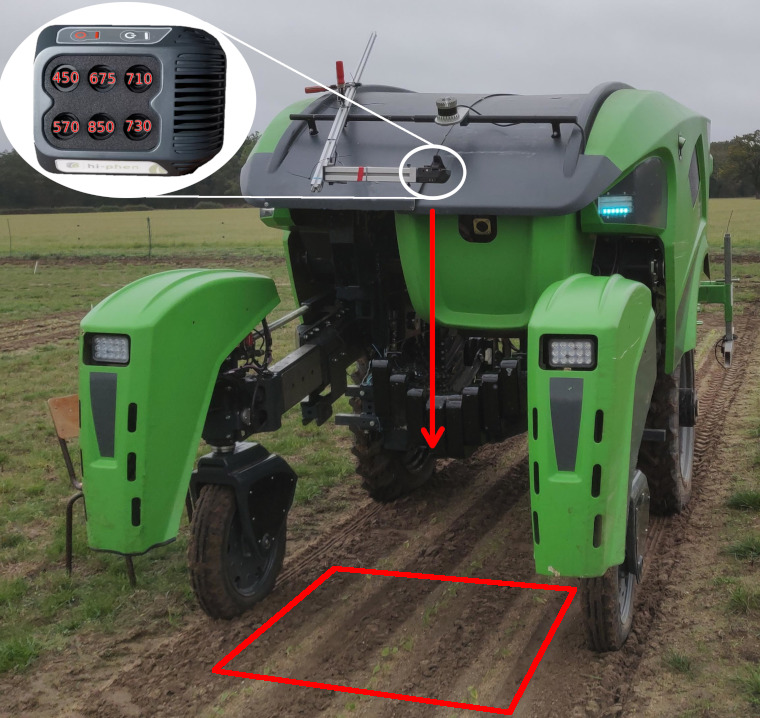
\includegraphics[height=3cm]{img/material/trektor}
        \caption{Robot et caméra utilisés par le consortium ROSEAU}
        \label{fig:04-robot-xp}
    \end{figure}
    
    %\colorbox{orange}{page a mal présenté par rapport à l'ancienne version}
    
    \newpage
    \subsection{Annotations}
    
    \subsubsection{Micro-parcelles}
    
    Les données acquises durant les expérimentations en micro-parcelles représentent un total de $1408$ images multispectrales. Chaque image a été annotée individuellement et manuellement pour la discrimination sol/végétation. Les annotations sont définies par des masques de segmentation binaire (noir = sol ou blanc = végétation).
    À titre d'illustration, la figure \ref{fig:04-mat-culture-adventice} montre à gauche une reconstruction en fausses couleurs d'une culture de maïs (dans un champ avec diverses mauvaises herbes et la présence d'ombres dans les coins de l'image) et montre à droite le masque de segmentation associé.
    
    \begin{figure}[H]
        \centering
        \adjincludegraphics[width=0.49\linewidth,trim={0 0 0 {0.1\height}},clip]{img/idx/false} \hfill
        \adjincludegraphics[width=0.49\linewidth,trim={0 0 0 {0.1\height}},clip]{img/idx/MASK}
        \caption{Fausses couleurs à gauche et vérité terrain manuelle correspondante à droite}
        \label{fig:04-mat-culture-adventice}
    \end{figure}
    
    Ces données n'ont pas été annotées pour la discrimination culture/adventices. En effet, au moment de leur acquisition, le choix du niveau de segmentation nécessaire et la définition des individus (pixel, composante connexe, plante, ou feuille) étaient en cours de discussion.
    
    \subsubsection{Challenge RoSE}
    
    Les acquisitions faites durant les challenges RoSE représentent 3443 images multispectrales. Dû à cette quantité et au temps nécessaire à leurs annotations seule une partie a été annotée. Les conditions propices (beau temps, sans vent) du challenge 2 et 3 ont permis de définir une base de données annotée de 300 images de haricots et de 92 images de maïs, pour la détection des feuilles. Ce qui n'a pas été le cas lors des challenges 4 et 5 (pluie et vent). En revanche, les mauvaises conditions ont été utilisées pour renforcer ``nos'' indices de végétations, que l'on présentera plus loin dans le chapitre \ref{chap:vegetation-indices}. Les annotations des feuilles ont été sous-traitées par la société Infolks (Inde) pour la partie haricot, et les annotations du maïs ont été faites en interne avec le logiciel VIA \cite{dutta2019vgg}. Ainsi, chaque feuille est associée à un polygone et à une étiquette (culture/adventice) comme représenté sur la figure suivante \ref{fig:04-mat-dataset-body}.
    
    \begin{figure}[H]
        \centering
        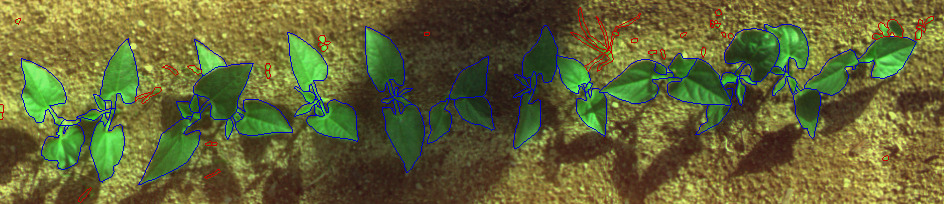
\includegraphics[width=\linewidth]{img/material/rose-gt-infolk}
        \caption{Annotation pour la discrimination des feuilles, entre culture et adventices}
        \label{fig:04-mat-dataset-body}
    \end{figure}
    
    \newpage
    
    \subsubsection{Autres jeux de données}
    
    \vspace{1em}
    Les algorithmes mis en place dans la suite de la thèse et notamment pour l'article intitulé \og Pixelwise Instance Segmentation Of Leaves In Dense Foliage \fg, ont nécessité des bases de données supplémentaires.
    
    Le premier jeu de données et a été fourni par le Réseau international sur le phénotypage des plantes (INPP) pour le Leaf Segmentation Challenge (LSC \cite{scharr2017computer}). Le jeu de données est en open-access. Il est composé d'images RGB de plantes Arabidopsis Thaliana (783 images) et de plantes de Rosette (27 images) segmentées en plusieurs feuilles (Figure \ref{fig:04-04-dataset-cvppp}). Les auteurs indiquent que les images ont été collectées à partir de plusieurs endroits dans une chambre de croissance expérimentale. Cette base de donnée est également acquis avec quatre caméras différentes et résolutions différentes.
    
    \begin{figure}[H]
        \centering
        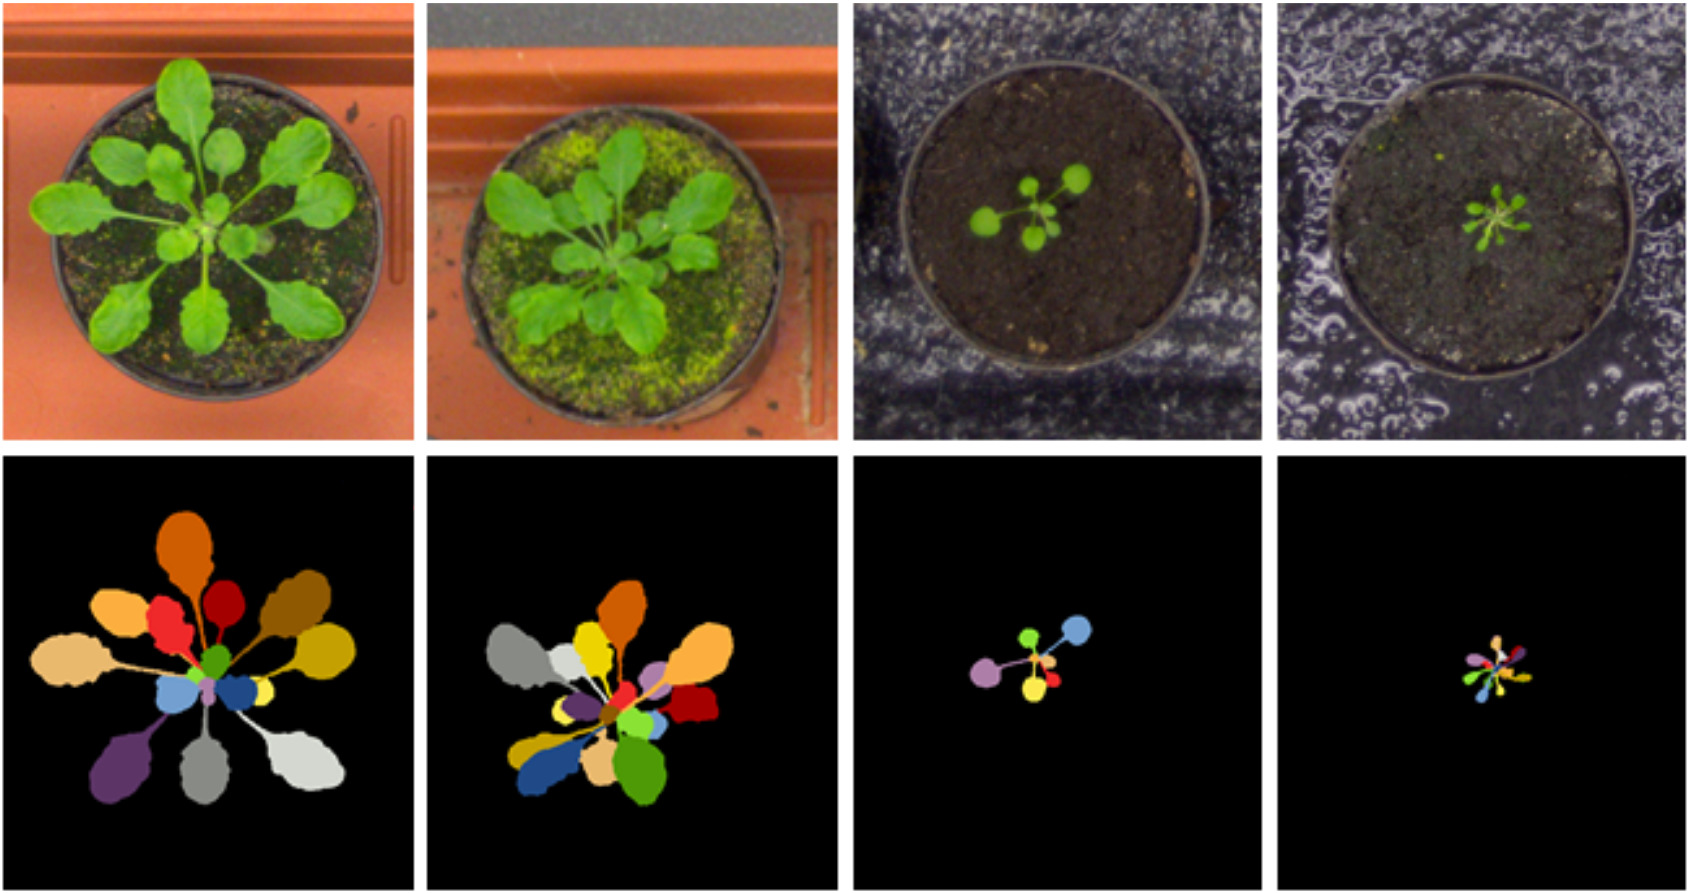
\includegraphics[width=0.8\linewidth]{img/leaf/dataset-cvppp}
        \caption{Exemples issues de la base de données CVPPP (haut) et vérité terrain (bas)}
        \label{fig:04-04-dataset-cvppp}
    \end{figure}
    
    Le deuxième jeu de données, Komatsuna, consiste en des images RGB de 137 plantes prises en vue de dessus. Ce jeu de données comprend 900 images de taille $480 \times 480$ pixels et contient un grand nombre de stades de croissance des plantes (138). Il a été conçu pour résoudre le problème du phénotypage 3D \cite{Uchiyama_2017_ICCV_Workshops}.
    
    \begin{figure}[H]
        \centering
        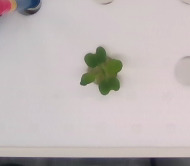
\includegraphics[width=0.2\linewidth]{img/leaf/dataset-Komatsuna-rgb-1}
        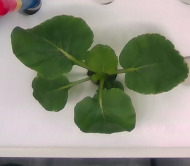
\includegraphics[width=0.2\linewidth]{img/leaf/dataset-Komatsuna-rgb-2}
        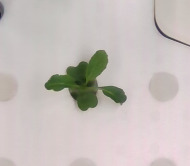
\includegraphics[width=0.2\linewidth]{img/leaf/dataset-Komatsuna-rgb-3}
        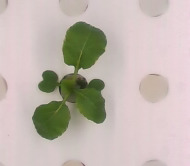
\includegraphics[width=0.2\linewidth]{img/leaf/dataset-Komatsuna-rgb-4} \\
        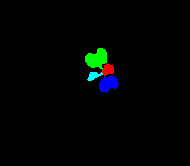
\includegraphics[width=0.2\linewidth]{img/leaf/dataset-Komatsuna-label-1}
        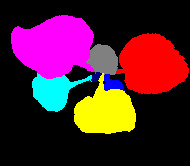
\includegraphics[width=0.2\linewidth]{img/leaf/dataset-Komatsuna-label-2}
        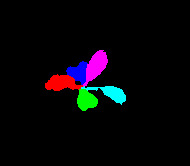
\includegraphics[width=0.2\linewidth]{img/leaf/dataset-Komatsuna-label-3}
        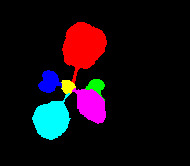
\includegraphics[width=0.2\linewidth]{img/leaf/dataset-Komatsuna-label-4} \\
        \caption{Exemples issues de la base de données Komatsuna (haut) et vérité terrain (bas)}
        \label{fig:04- }
    \end{figure}
    
    \newpage
    \section{Calibration}
    
    \subsection{Résolution spatiale}
    
    La caméra multispectrale Airphen est habituellement dédiée à des applications drone avec une optique optimisée pour des vols supérieurs à \SI{25}{m} d'altitude. Dans le cadre du challenge RoSE, cette caméra est destinée à être fixée en amont du robot terrestre. La fauchée ou emprise au sol de l'image, représentée par le rectangle projeté, sur la figure \ref{fig:04-camera-distance-sol}, est fonction de l'altitude, de la taille du capteur et de la distance focale.
    
    \vfill
    \begin{figure}[H]
        \centering
        %\source{\cite{lisein:tel-01539627}}
        \begin{minipage}[b]{0.60\linewidth}
            \centering
            %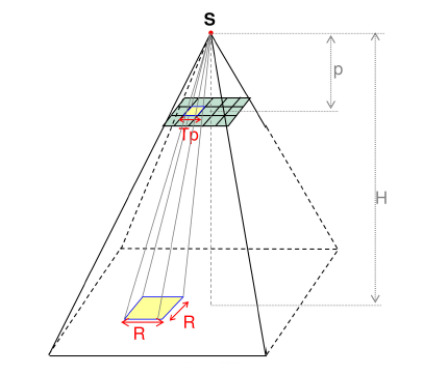
\includegraphics[width=\linewidth]{img/material/camera-distance-sol}
            
\begin{tikzpicture}[scale=.7,every node/.style={minimum size=1cm},on grid]
	% bottom part
	\begin{scope}[yshift=-83,every node/.append style={yslant=0.5,xslant=-1},yslant=0.5,xslant=-1, scale=2.5]
		\fill[top color=black!5, bottom color=white] (0,0) rectangle (2,2);
		\draw[step=4mm, black] (0,0) grid (2,2); 
		\draw[black,thick] (0,0) rectangle (2,2);
		% center pixel
		\fill[top color=black!10, bottom color=orange] (0.85,0.85) rectangle (1.15,1.15);
		% upper part
		\fill[top color=black!10, bottom color=yellow] (1.25,0.85) rectangle (1.55,1.15);
		\fill[top color=black!10, bottom color=yellow] (0.85,1.25) rectangle (1.15,1.55);
		\fill[top color=black!10, bottom color=yellow] (1.25,1.25) rectangle (1.55,1.55);
		% lower part
		\fill[top color=black!10, bottom color=yellow] (0.45,0.85) rectangle (0.75,1.15);
		\fill[top color=black!10, bottom color=yellow] (0.85,0.45) rectangle (1.15,0.75);
		\fill[top color=black!10, bottom color=yellow] (0.45,0.45) rectangle (0.75,0.75);
		left and right
		\fill[top color=black!10, bottom color=green] (0.45,1.25) rectangle (0.75,1.55);
		\fill[top color=black!10, bottom color=yellow] (1.25,0.45) rectangle (1.55,0.75);
		% dim
		\draw[<->,] (-0.05, 1.20) to (-0.05,1.6);
		\node (R) at (-0.15, 1.40) {R};
		\draw[<->,] (1.20,-0.05) to (1.6,-0.05);
		\node (R) at (1.40,-0.15) {R};
		
		%\foreach \i in {1,...,300}{
		%	\fill [black, fill opacity=0.3] (rnd*2,rnd*2) circle [radius=0.2pt];
		%}
	\end{scope}
	
	% triangle
	%\draw[-, dashed] ( 0,-2.93) to (0,6);
	\draw[-, dashed] (-5,-0.38) to ( 2,6.1);
	\draw[-, dashed] ( 5,-0.38) to (-2,6.1);
	%\draw[-, dashed] ( 0,4.25) to ( 0,6.1);
	\draw[-, dashed] ( 0,-2.93) to ( 0,7.1);
	
	% square projection
	\draw[-, dotted] (-1.29,-0.41) to (0.5,6.1);
	\draw[-, dotted] (-2.75,-0.41) to (1.1,6.1);
	\draw[-, dotted] (-2.00,-0.79) to (0.8,6.25);
	\draw[-, dotted] (-2.00,-0.04) to (0.8,5.95);
	
	% upper part
	\begin{scope}[yshift=145,every node/.append style={yslant=0.5,xslant=-1},yslant=0.5,xslant=-1]
		\fill[black!5,fill opacity=0.5] (0,0) rectangle (2,2);
		\draw[step=4mm, black] (0,0) grid (2,2); 
		\draw[black,thick] (0,0) rectangle (2,2);
		% center pixel
		\fill[orange] (0.85,0.85) rectangle (1.15,1.15);
		% upper part
		\fill[yellow] (1.25,0.85) rectangle (1.55,1.15);
		\fill[yellow] (0.85,1.25) rectangle (1.15,1.55);
		\fill[yellow] (1.25,1.25) rectangle (1.55,1.55);
		% lower part
		\fill[yellow] (0.45,0.85) rectangle (0.75,1.15);
		\fill[yellow] (0.85,0.45) rectangle (1.15,0.75);
		\fill[yellow] (0.45,0.45) rectangle (0.75,0.75);
		left and right
		\fill[yellow] (0.45,1.25) rectangle (0.75,1.55);
		\fill[green] (1.25,0.45) rectangle (1.55,0.75);
		% dim
		\draw[<->,] (2.15, 1.20) to (2.15,1.6);
		\node (P) at (2.45, 1.40) {P};
		\draw[<->,] (1.20,2.15) to (1.6,2.15);
		\node (P) at (1.40,2.45) {P};
	\end{scope}
	
	%heigh
	\draw[-, dotted] (0,6.1) to (6,6.1);
	\draw[-, dotted] (0,4.25) to (6,4.25);
	\draw[-, dotted] (0,-0.4) to (6,-0.4);
	\draw[-latex,thick,<->,] (6,-0.4) to (6,4.25);
	\draw[-latex,thick,<->,] (6,4.25) to (6,6.1);
	\node (F) at (5.7,5.175) {F};
	\node (H) at (5.7,2.125) {H};
	\node (C) at (-0.5,4.25) {C};
	
	% points
	\fill[blue] (0,6.1) circle (2pt);
	\fill[blue] (0,4.25) circle (2pt);
	\fill[blue] (0,-0.4) circle (2pt);
	
	\draw[-latex,thick](-3.2,1.5) node[left]{\small Scene}
	to[out=0,in=135] (-1.95,1.05);
	\draw[-latex,thick,](-3,5) node[left]{\small Image}
	to[out=0,in=225] (-1.2,5.7);

\end{tikzpicture}
        \end{minipage}%
        \hspace{-1cm}
        \begin{minipage}[b]{0.35\linewidth}
            \centering
            \noindent
            \begin{itemize}
                \item C : Centre optique
                \item H : Hauteur de la caméra
                \item F : Distance focale
                \item P : Taille du photosite
                \item R : Résolution spatiale
                \item R = ${H} \times P \div F$.
            \end{itemize}
            \vspace{2cm}
        \end{minipage}%
        \caption{Relation entre paramètres du monde réel et ceux du monde virtuel}
        \label{fig:04-camera-distance-sol}
    \end{figure}
    \vfill
    
    À titre indicatif, le tableau suivant \ref{tab:04-acquisition-resolution} montre les largeurs et longueurs de la zone observée par cette caméra en fonction de la hauteur. La résolution spatiale des pixels en millimètres est également renseignée. À basse altitude, la résolution des images est haute, a contrario plus la hauteur augmente, plus la zone observée est grande et plus la résolution spatiale des pixels est faible. Ainsi, à \SI{1.80}{m} d'altitude, la zone observée est de $\SI{1.08}{m} \times \SI{0.81}{m}$ avec une résolution spatiale des pixels de $\SI{0.84}{mm^2/px}$. Ce qui permet d'observer les rangs de culture, tout en prenant une marge d'erreur sur les bords, nécessaire entre autres au recalage des images multispectrales.
    
    \vfill
    \begin{table}[H]
        \centering
        \rowcolors{0}{gray!10}{white}
        \begin{tabular}{| l | c c c c c c c c c c c | r |}  \hline
            \textbf{Hauteur}  & 1.00 & 1.20 & 1.40 & 1.60 & 1.80 & 2.00 & 2.20 & 2.40 & 2.60 & 2.80 & 3.00 & \textbf{Unité} \\ \hline
            \textbf{Longueur} & 0.45 & 0.54 & 0.63 & 0.72 & 0.81 & 0.90 & 0.99 & 1.08 & 1.17 & 1.26 & 1.35 & $m$\\
            \textbf{Largeur}  & 0.60 & 0.72 & 0.84 & 0.96 & 1.08 & 1.20 & 1.32 & 1.44 & 1.56 & 1.68 & 1.80 & $m$ \\ \hline
            \textbf{Résolution} & 0.47 & 0.56 & 0.66 & 0.75 & 0.84 & 0.94 & 1.03 & 1.12 & 1.22 & 1.31 & 1.41 & $mm^2/px$ \\ \hline
        \end{tabular}
        \caption{Résolution spatiale des images à différentes hauteurs}
        \label{tab:04-acquisition-resolution}
    \end{table}
    \vfill
    
    \newpage
    \subsection{Correction géométrique}
    \label{sec:acquisition-calibration-lens}
    
    Comme nous l'avons vu dans le chapitre précédent, à la section \ref{sec:lens-correction}, l'une des premières source d'erreur est issue de l'alignement du capteur et de la lentille. Le fournisseur de la caméra Airphen ne propose pas de calibration des lentilles, une correction de ces dernières (6 capteurs optiques) a été faite pour corriger les déformations visuellement perceptibles. Chaque capteur dispose d'une lentille dont les spécifications sont identiques entres elles, mais peuvent légèrement différer en sortie de fabrication. Pour détecter les déformations, un échiquier calibré a été photographié sous différents angles de vue (figure \ref{fig:04-echiquier}). Ainsi 204 images ont été acquises pour chaque longueur d'onde.
    
    \begin{figure}[H]
        \centering
        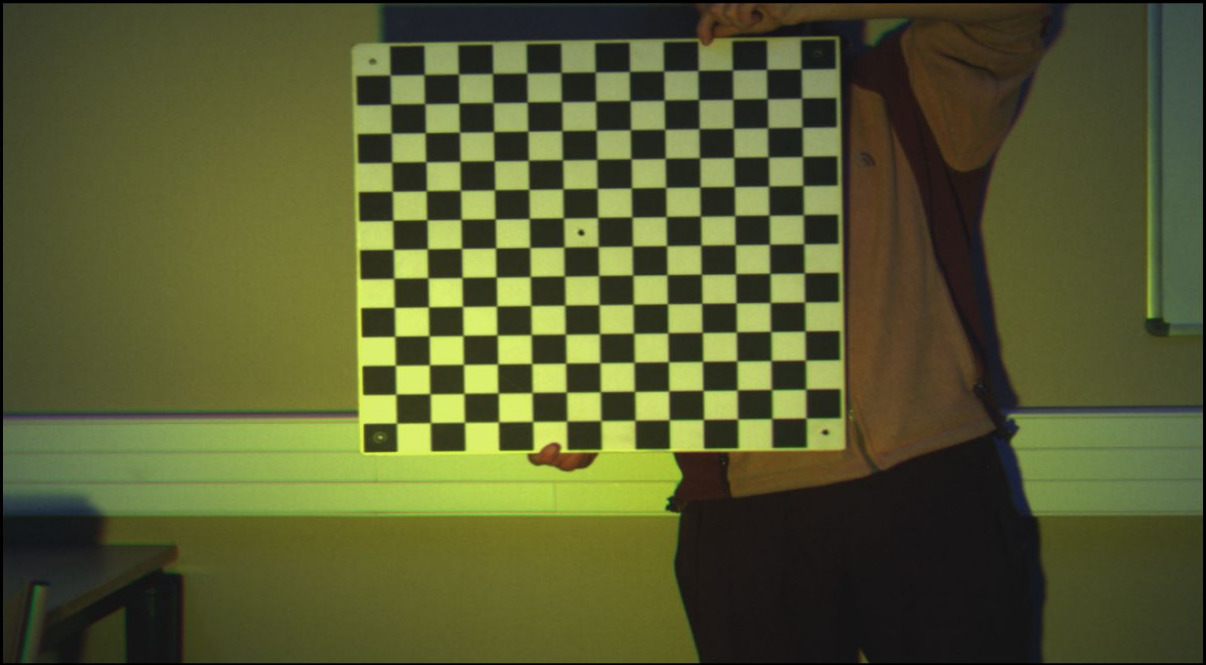
\includegraphics[height=2.5cm]{img/preprocessing/echiquier}
        \caption{Échiquier de calibration géométrique}
        \label{fig:04-echiquier}
    \end{figure}
    
    Le modèle standard de distorsion est obtenu par l'ajout de la distorsion tangentielle aux modèles de distorsion radiale et d'un modèle de distorsion prismatique \cite{Wang:2008:NCM:1294369.1294525}. La fonction  $\Phi$ ci-dessous \eqref{eq:lens-distortion} définit le mappage polynomial $2D\rightarrow2D$ du modèle de distorsion.
    
    \begin{equation}
    %\left(\begin{matrix} x_u \\ y_u \end{matrix}\right)
    %=
    \Phi
    \left(\begin{matrix} x_d \\ y_d \end{matrix}\right)
    =
    \left(\begin{matrix}
    x_d\,(1 + k_1 r^2 + k_2 r^4 + k_3 r^6) + 2 p_1 x_d y_d + p_2 (r^2 + 2 x_d^2) + s_1 r^2 + s_2 r^4 \\
    y_d\,(1 + k_1 r^2 + k_2 r^4 + k_3 r^6) + 2 p_2 x_d y_d + p_1 (r^2 + 2 y_d^2) + s_3 r^2 + s_4 r^4
    \end{matrix}\right)
    \label{eq:lens-distortion}
    \end{equation}
    
    \par Où $r^2 = x_d^2+y_d^2$, $(x_d,y_d)^t$ sont les coordonnées distordues et normalisées. La fonction $\Phi$ donne en sortie les coordonnées image normalisées corrigées, notées $(x_u,y_u)^t$. Les coordonnées image normalisées sont calculées par translation du centre optique et divisées par la profondeur de la focale en pixel. Ainsi, $(x_u,y_u)^t$ et $(x_d,y_d)^t$ sont indépendants de la dimension de l'image. Nous pouvons aussi réécrire l'équation de façon plus explicite, pour séparer les différents modèles :
    
    \begin{eqnarray}
    \begin{array}{rlcccccc}
    x_u &= x_d &+& {x_d(k_1 r^2 + k_2 r^4 + k_3 r^6)}
    &+& {2 p_1 x_d y_d + p_2(r^2 + 2 x_d^2)}
    &+& {s_1 r^2 + s_2 r^4} \\
    
    y_u &= y_d &+& {\underbrace{y_d(k_1 r^2 + k_2 r^4 + k_3 r^6)}}
    &+& {\underbrace{2 p_2 x_d y_d + p_1(r^2 + 2 y_d^2)}}
    &+& {\underbrace{s_3 r^2 + s_4 r^4}} \\
    
    &      & & {\Delta {radial}}
    &+& {\Delta {tangential}}
    &+& {\Delta {prism}}
    \end{array}
    \end{eqnarray}
    
    \par Il existe plusieurs outils pour chercher et estimer cette fonction, afin d'effectuer la rectification de la distorsion. La calibration a ainsi été réalisée avec OpenCV, et ce, pour chaque lentille de façon indépendante. Il existe donc 6 fonctions de mappage $\Phi$. Après calibration, on peut calculer l'erreur de re-projection, exprimée en pixel. Pour ce faire, on calcule la moyenne des distances euclidiennes entre les points détectés et ceux calibrés et reprojetés. Les résultats sont visibles sur le tableau \ref{tab:04-geom-error}.
    
    \begin{table}[H]
        \centering
        \rowcolors{0}{gray!10}{white}
        \begin{tabular}{|l|c|c|c|c|c|c|}
            \hline
            \textbf{Bande Spectrale} & \SI{450}{nm} & \SI{570}{nm} & \SI{675}{nm} & \SI{710}{nm} & \SI{730}{nm} & \SI{850}{nm} \\ \hline
            \textbf{Erreur Résiduelle} & \SI{0.0115}{px} & \SI{0.0092}{px} & \SI{0.0096}{px} & \SI{0.0094}{px} & \SI{0.0092}{px} & \SI{0.0110}{px} \\
            \hline
        \end{tabular}
        \caption{Erreur résiduelle, en pixel, après correction géométrique}
        \label{tab:04-geom-error}
    \end{table}
    
    \newpage
    \paragraph{Exemple} À titre indicatif, les paramètres de déformation de la fonction $\Phi$ estimés pour la bande \SI{450}{nm} sont visibles sur le tableau \ref{tab:04-geom-450}. Et la figure \ref{fig:04-geom-450-lens-correction} montre les différentes corrections. De haut en bas : prismatique, tangentiel et radial de la bande \SI{450}{nm}. On constate ici que pour la bande \SI{450}{nm} la correction prismatique est négligeable. À contrario, les variables pour la correction radiale (k1 et k2) et tangentielle (p2) montrent des rectifications importantes.
    
    \vfill
    \begin{table}[H]
        \centering
        \rowcolors{0}{gray!10}{white}
        \begin{tabular}{|l|l|l|}
            \hline
            \textbf{Correction} & \textbf{Variables} & \textbf{Valeurs} \\
            \hline
            radial 		& k1,k2,k3 		& -0.55181 ;  0.30429 ; -0.00053 \\
            prism  		& s1,s2,s3,s4	&  0.03471 ;  0.01294 ;  0.0025 ; -0.00183 \\
            tangential 	& p1,p2 		&  0.00267 ; -0.43599 \\
            \hline
        \end{tabular}
        \caption{Correction de la lentille pour la bande spectral \SI{450}{nm}}
        \label{tab:04-geom-450}
    \end{table}
    \vfill
    \begin{figure}[H]
        \centering
        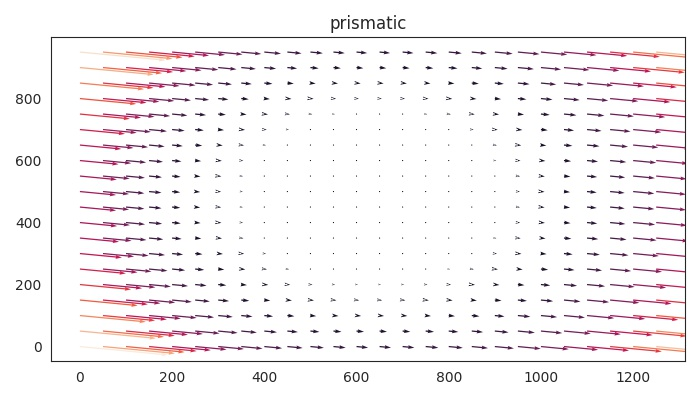
\includegraphics[width=0.6\linewidth]{img/preprocessing/lens-correction-prismatic}
        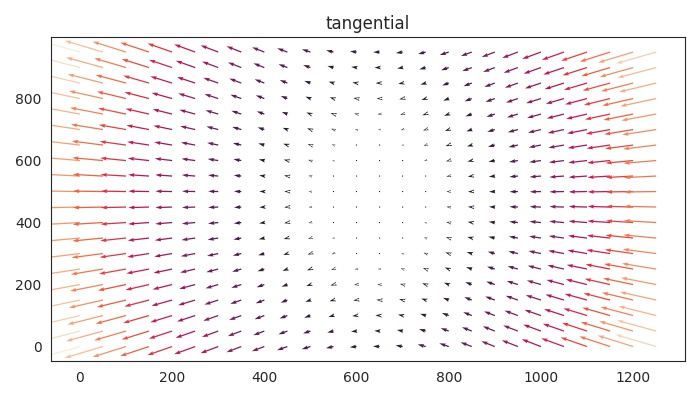
\includegraphics[width=0.6\linewidth]{img/preprocessing/lens-correction-tangential}
        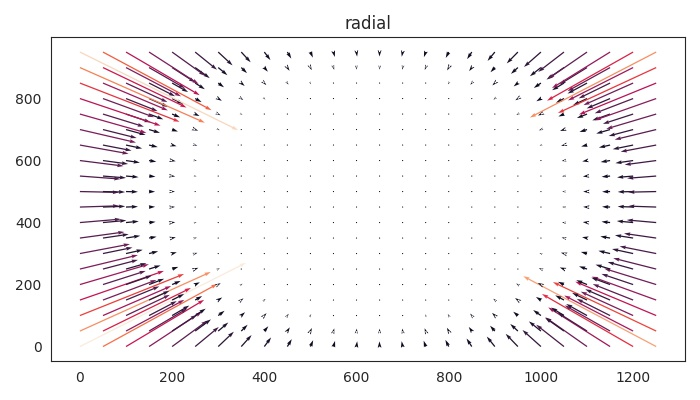
\includegraphics[width=0.6\linewidth]{img/preprocessing/lens-correction-radial}
        \caption{Visualisation de la correction géométrique pour la bande \SI{450}{nm}}
        \label{fig:04-geom-450-lens-correction}
    \end{figure}
    \vfill
    
\end{document}